\documentclass[journal=jmcmar,manuscript=article]{achemso}


%%%%%%%%%%%%%%%%%%%%%%%%%%%%%%%%%%%%%%%%%%%%%%%%%%%%%%%%%%%%%%%%%%%%%
%% Place any additional packages needed here.  Only include packages
%% which are essential, to avoid problems later. Do NOT use any
%% packages which require e-TeX (for example etoolbox): the e-TeX
%% extensions are not currently available on the ACS conversion
%% servers.
%%%%%%%%%%%%%%%%%%%%%%%%%%%%%%%%%%%%%%%%%%%%%%%%%%%%%%%%%%%%%%%%%%%%%
\usepackage[version=3]{mhchem} % Formula subscripts using \ce{}
\usepackage{subcaption}
\usepackage{array}
\usepackage{url}
\usepackage{xr-hyper}
\usepackage{hyperref}
\usepackage{multirow}
\usepackage{listings}
\usepackage[flushleft]{threeparttable}
%\captionsetup[figure]{font=small,labelfont=small}

\makeatletter
\newcommand*{\addFileDependency}[1]{% argument=file name and extension
  \typeout{(#1)}
  \@addtofilelist{#1}
  \IfFileExists{#1}{}{\typeout{No file #1.}}
}
\setlength\acs@tocentry@height{8.25cm}
\setlength\acs@tocentry@width{4.45cm}
\makeatother
\newcommand*{\myexternaldocument}[1]{%
    \externaldocument{#1}%
    \addFileDependency{#1.tex}%
    \addFileDependency{#1.aux}%
}

%\myexternaldocument{supp}
\newcommand*\mycommand[1]{\texttt{\emph{#1}}}


\title{SolTranNet -- A ML tool for fast aqueous solubility prediction.}
\keywords{deep learning, machine learning, molecular property prediction, solubility, tool}
\author{Paul G. Francoeur}
\author{David R. Koes}
\email{dkoes@pitt.edu}
\affiliation[Pitt]{Department of Computational and Systems Biology, University of Pittsburgh, Pittsburgh, PA 15260}
\date{August 2020}

\begin{document}
%%%%%%%%%%%%%%%%%%%%%%%%%%%%%%%%%%%%%%%%%%%%%%%%%%%%%%%%%%%%%%%%%%%%%
%% The abstract environment will automatically gobble the contents
%% if an abstract is not used by the target journal.
%%%%%%%%%%%%%%%%%%%%%%%%%%%%%%%%%%%%%%%%%%%%%%%%%%%%%%%%%%%%%%%%%%%%%
\begin{abstract}
To Be Written upon completion of the rest of the draft

\end{abstract}

%%%%%%%%%%%%%%%%%%%%%%%%%%%%%%%%%

%%%%%%%%%%%%%%%%%%%%%%%%%%%%%%%%%%%%%%%%%%%%%%%%%%%%%%%%%%%%%%%%%%%%%
%% Introduction and Background
%%%%%%%%%%%%%%%%%%%%%%%%%%%%%%%%%%%%%%%%%%%%%%%%%%%%%%%%%%%%%%%%%%%%%
\section{Introduction}
Aqueous solubility is an important physiochemical property for drug discovery, in part due to humans being 60\% water\cite{HumanWater} and absorption through the intestinal tract being a common form of drug delivery. 
In addition to simple absorption into the body, the drug's behavior in water is also linked to how it moves throughout the body and is eliminated. Each of these properties are potential causes of failure in the drug discovery pipeline, which renders aqueous solubility to be one of the most important properties of a given drug.\cite{LIPINSKI1997,DI2006446,EKINS2002305}
Traditionally, one would directly measure the solubility of a given compound.
However, such an approach is slow, expensive, and requires some amount of the compound to be available for the experiments.
With the increasing size of molecular screening libraries, up to 350 million compounds,\cite{NatureVS} experimentally measuring the solubility of each compound becomes impossible.
Thus there is a need for fast and accurate solubility prediction for a given molecule.

Predicting aqueous solubility for a given molecule is typically performed with one of three methods: molecular simulation, quantum calculations, or through the use of an empirically fit function.
Molecular simulation approaches utilize statistical mechanics and either directly calculate the solubility from the chemical potentials of the solute and water\cite{denseStates}, or directly simulate the solute in a bulk of water molecules.
For direct simulation of the solute, there are several methods available as reviewed by \citet{solrev1}.
However, each of these approaches use a large amount of computing power, and in the case of direct simulation also require a long time to reach equilibrium.

Quantum mechanics (QM) based approaches are more accurate than the simulation approach, and can be divided into two broad categories based on if the solvent is included in the calculation. 
Full QM methods include the water molecules in their calculations and are based on density functional theory\cite{solrev1}.
This approach is the most correct model, but still suffers from underestimating the equilibrium density of the solute, and requires the most computing power.
On the other hand, continuum of the solvent methods treat the water as a bulk dielectric.
This saves on computing power at the cost of not sampling the degrees of freedom of the water molecules and assuming that the solute's charge is entirely contained in the cavity it creates in the solvent.

Both of the previous methods require a large amount of computing power in order to perform their calculations.
In order to avoid this, there has been extensive work in creating empirical models for solubility prediction\cite{solrev1,solrev2}.
These empirical methods all utilize some set of molecules with known solubility as training data, and then fit a function based on features of the molecules in the training data to predict the solubility.
This approach is much faster, but fails to generalize to molecules outside of scope of the molecules represented in the training set.
As in many other applications, machine learning (ML) approaches have been supplanting the traditionally fit functions for this empirical approach.
Indeed, all of the approaches in the second challenge to predict aqueous solubility utilized some form of ML algorithm.\cite{llinas}
\citet{boobier} found that typical ML algorithms performed equally as well as human experts for predicting the solubility of drug-like compounds.
\citet{lovric} performed a study of several ML methods, and showed that simpler ML approaches generalized better to unseen data, and proposed selecting a method based on a combination of its own test set performance, ability to generalize, and number of features.
Deeper models have also shown improvement at this task, as shown by \citet{cui}, who utilized a 20 layer modified ResNet convolutional neural network architecture.
\citet{MAT} developed the molecular attention transformer (MAT) architecture, which is modeled after the current state of the art transformer architecture for language processing.
MAT was utilized for a variety of molecular property prediction tasks, and performed well at solubility prediction although not being particularly optimized for this task.

Here we present SolTranNet, a ML model based on the MAT architecture, for predicting aqueous solubility.
We trained SolTranNet utilizing the AqSolDB dataset\cite{AqSol}, as it was the largest publicly available curated set, and optimized it for both speed and quality of prediction.
SolTranNet had an INSERT $R^2$ and INSERT root mean square error (RMSE) on clustered cross-validation splits of AqSolDB.
We also compare to other recently published ML models.\cite{lovric,cui,boobier,llinas}
SolTranNet is available via pip installation for python3, and the source code, datasets, and documentation are available at (insert git repo).


%%%%%%%%%%%%%%%%%%%%%%%%%%%%%%%%%%%%%%%%%%%%%%%%%%%%%%%%%%%%%%%%%%%%%
%% Methods
%%%%%%%%%%%%%%%%%%%%%%%%%%%%%%%%%%%%%%%%%%%%%%%%%%%%%%%%%%%%%%%%%%%%%
\section{Methods}

\subsection{Datasets}
The main dataset we utilized for training SolTranNet is AqsolDB\cite{AqSol}, which was selected as it was the largest publicly available set.
Notably, while there are many other features available in AqsolDB, we only utilized the SMILES string, and the reported solubility (logS, where S is in mol/L).
We then utilized rdkit\cite{rdkit} to calculate the Murcko scaffolds of the molecules, which were then utilized to cluster the molecules and generate a 3 fold clustered cross-validation (CCV) split of the data.
We additionally created an independent test set out of the molecules present in the Solubility Challenge 2 test sets \cite{llinas} and FreeSolv \cite{freesolv}, such that no molecule in the independent test set has an rdkit fingerprint similarity of greater than or equal to 0.9 to any molecule in AqSolDB.
The histograms of each fold of the scaffold split as well as the full AqSolDB set and our independent set are shown in SFig(ref)
The CCV AqSolDB dataset, and our independent test set were utilized to optimize SolTranNet's final architecture, as described in the Model Selection search subsection.

While the provided sets above allow for an evaluation of SolTranNet, we also seek to compare to other published models. Given that we created our own test set, we seek to evaluate both our deployed model as well as the training procedure we utilized to select it on other published sets.
\citet{boobier} provided a training and testing set (75 and 25 molecules respectively) utilized in 2017 which showed ML models performing equally as well as human experts.
\citet{cui} provided a training set of 9943 molecules and a testing set of 62 molecules that they utilized to evaluate a deep ResNet based ML model.
\citet{lovric} provided a set of 829 molecules which they randomly split into a training, validation, and testing set consisting of 64\%, 16\%, and 20\% of the molecules respectively.
This set was utilized to test various ML algorithms for their ability to predict aqueous solubility.
Lastly, \citet{llinas} hosted the second solubility challenge, wherein two test sets were provided and participants could utilize any training set they desired, provided that no molecule was present in the test sets.
As such, we filtered AqSolDB such that there was no overlap with any molecule present (as determined by a Tanimoto similarity of 1 between the default rdkit fingerprint's of each molecule in AqSolDB and provided by \citet{llinas}) in the second solubility challenge to use as a new training set.

\subsection{Model Selection Search}
The general architecture of the MAT model is provided in Figure\ref{fig:architecture}.
In order to optimize the hyper-parameters for SolTranNet, we utilized a 2 stage optimization procedure as shown in Table\ref{tab:wandsweep}.
All hyperparameter optimizations were performed utilizing the Weights and Biases platform\cite{wandb}.
The first stage of the sweep was a hyperband search over the hyperparameters regarding the model's optimizer, as well as the learning rate, and which loss function was utilized as shown in Table\ref{tab:initsweep}. The goal of the search was to minimize the RMSE of the test set for the first fold of the CCV scaffold split of AqSolDB.
This resulted in utilizing the huber loss function, a 2D embedding for the molecules, and the stochastic gradient descent (SGD) optimizer with momentum of 0.06, no weight decay, and with a learning rate of 0.04.
After this stage was completed, we then performed a grid search over the particular hyperparameters regarding SolTranNet itself for 100 epochs over each fold of the CCV scaffold split of AqSolDB as shown in Table\ref{tab:archsweep}.

\begin{figure}[tb]
    \centering
    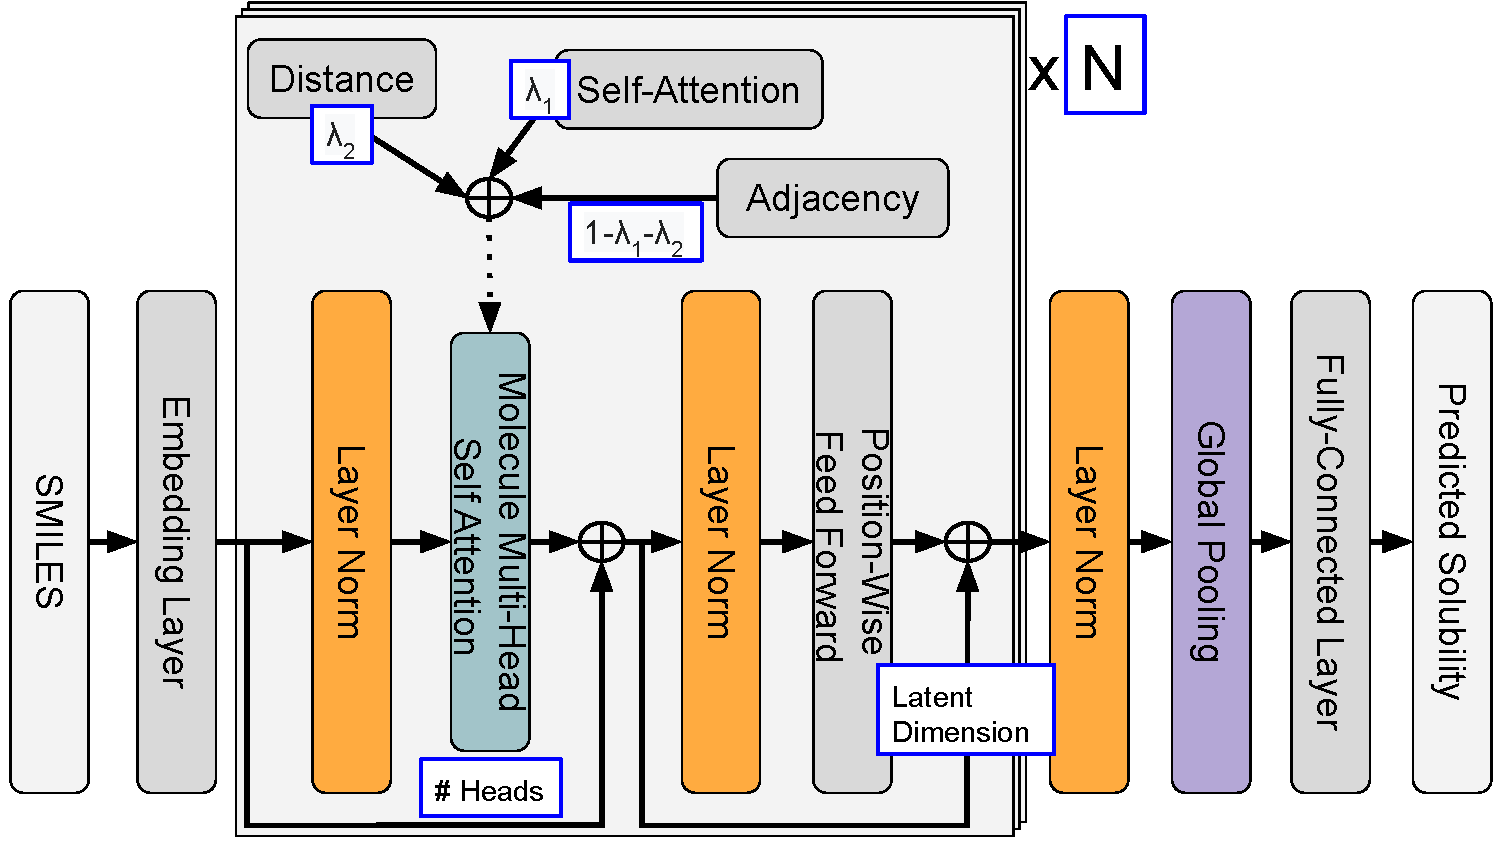
\includegraphics[width=\linewidth]{figure/soltrannet_architecture.pdf}
    \caption{General Architecture of SolTranNet. Each item in a blue box is a tuned hyperparameter, whose values were tested as shown in Table\ref{tab:archsweep}.}
    \label{fig:architecture}
\end{figure}

\begin{figure}[tb]
    \subfloat[Optimizer Hyperband Sweep]{
        \centering
        \begin{tabular}{|c|c|}
        \hline
            Parameter & Range \\
        \hline
            Training Epochs & [250, 2000]  \\
            Loss Function & MSE, MAE, Huber  \\
            Learning Rate & [0.0001, 0.1]  \\
            Momentum & [0.5, 0.9]  \\
            Optimizer & SGD, Adam  \\
            Weight Decay & [0, 0.5]  \\
            Dimension of Conformer Generation & 2D, 3D  \\
            Scaffold CCV fold & 0 \\
            Target & minimize test RMSE  \\
        \hline
        \end{tabular}
        \label{tab:initsweep}
    }
    
    \subfloat[Architecture Grid Search]{
        \centering
        \begin{tabular}{|c|c|}
        \hline
            Parameter & Range \\
        \hline
             Latent Dimension of Encoder & 2, 4, \textbf{8}, 16, 32, 64, 128, 256, 512, 1024  \\
             Dropout & 0, \textbf{0.1}  \\
             Number of Attention Heads & \textbf{2}, 4, 8, 16, 32  \\
             $\lambda_1$ Attention & 0.25, 0.33, \textbf{0.5}  \\
             $\lambda_2$ Distance & \textbf{0}, 0.33  \\
             Number of Encoder Stacks & 2, 4, 6, \textbf{8}, 16  \\
             Scaffold CCV folds & 0, 1, 2  \\
             Loss Function & Huber  \\
             Learning Rate & 0.04  \\
             Momentum & 0.06  \\
             Optimizer & SGD  \\
             Weight Decay & 0  \\
         \hline
        \end{tabular}
        \label{tab:archsweep}
    }
    \caption{Two stage hyperparameter sweep for SolTranNet. The Optimizer sweep was performed via using Weights and Bias's hyperband sweeping tool, with the target to minimize the test set RMSE. The Architecture sweep was a grid search over the listed parameters after the optimizer hyperparameters were set from the first stage. The deployed version of SolTranNet uses the hyperparameters in bold.}
    \label{tab:wandsweep}
\end{figure}

In order determine which version of the model was performing the best, we calculated the $R^2$ and the root mean square error (RMSE) of the predicted solubility.
Since AqSolDB, as well as several other solubility datasets, span several orders of magnitude, the $R^2$ correlation metric is easier to perform well on.
Thus, we selected our best performing model by its RMSE performance on our independent test set.
Additionally, as we intend for this tool to be deployed for use on potentially very large datasets, we took into account the speed of SolTranNet in our hyperparameter search.
This speed analysis really only had an effect on the decision to utilize a 2D embedding of the conformer generation, and only have 1 densely connected layer as the final layer of the network.

\subsection{Final model training}
The final architecture of SolTranNet utilized the following hyperparameters: 0.1 dropout, 0 lambda distance, 0.5 lambda attention, 1 final dense layer, 2 attention heads, a hidden dimension of size 8, and 8 stacks in the transformer encoding layer.
The molecular embedding layer was unchanged from the initial MAT implementation\cite{MAT} where each atom is represented via a node with a feature vector as shown in SFig\ref{tab:atomembed}.
In order to select the final deployed model, we trained 5 models with different random seeds on all of the data in AqSolDB utilizing the huber loss function, the SGD optimizer with momentum of 0.06, no weight decay, and with a learning rate of 0.04.
We dynamically stopped training based on failing to improve fit to the training set for 4 epochs.
After training stopped, we deployed the model with the best RMSE and $R^2$ performance on our independent test set without being an outlier as shown in SFig\ref{fig:dynsweep}.

%%%%%%%%%%%%%%%%%%%%%%%%%%%%%%%%%%%%%%%%%%%%%%%%%%%%%%%%%%%%%%%%%%%%%
%% Results
%%%%%%%%%%%%%%%%%%%%%%%%%%%%%%%%%%%%%%%%%%%%%%%%%%%%%%%%%%%%%%%%%%%%%
\section{Results}

\subsection{final model sweep/selection}
\begin{table}
    %\centering
    \begin{tabular}{|c|c|c|c|c|c|c|}
        \hline
         Model & Parameters & CCV RMSE & Fold0 RMSE & Fold1 RMSE & Fold2 RMSE & Ind RMSE \\
         \hline
         MAT & 42,049,537 & 2.007 & 1.231 & 3.075 & 1.058 & 2.113  \\
         \hline
         0 & 21,061,633 & 1.449 & 1.161 & 1.959 & 1.054 & 1.914 \\
         1 & 502,529 & 1.467 & 1.231 & 1.972 & 1.028 & 1.946 \\
         2 & 336,385 & 1.377 & 1.260 & 1.682 & 1.126 & 1.870 \\
         3 & 336,385 & 1.454 & 1.239 & 1.857 & 1.165 & 1.949 \\
         4 & 22,657 & 1.297 & 1.187 & \textbf{1.582} & 1.066 & 1.903 \\
         5 & 11,905 & \textbf{1.271} & \textbf{1.130} & 1.605 & \textbf{0.998} & 1.923 \\
         6 & 11,905 & 1.350 & 1.272 & 1.680 & 1.012 & 1.903\\
         \emph{7} & \emph{3,393} & \emph{1.459} & \emph{1.172} & \emph{1.916} & \emph{1.159} & \emph{\textbf{1.779}}\\
         8 & 2,609 & 1.376 & 1.169 & 1.788 & 1.055  & 1.973 \\
         9 & 2,609 & 1.454 & 1.252 & 1.919 & 1.043  & 1.973 \\
         \hline
         Elastic & 1,463 & 1.835 & 1.843 & 1.965 & 1.687  & 2.090\\
         Lasso & 1,077 & 1.876 & 1.914 & 1.984 & 1.719 & 2.136\\
         PLS & 2,048 & 2.413 & 3.085 & 2.082 & 1.902 & 2.081\\
         Ridge & 2,048 & 2.239 & 2.503 & 2.032 & 2.155 & 2.312 \\
         \hline
    \end{tabular}
    \caption{SolTranNet model hyperparameter search for predicting solubility RMSE. Additionally, all models outperform linear approaches. The model in italics is the final model selection. There is a potential peak of model performance with the deployed model.}
    \label{tab:solsearchrmse}
\end{table}

new table input

\subsection{Architecture Train Aqsol test IND}

\begin{table}
    \begin{tabular}{|c|c|c|c|c|}
        Model & Train RMSE & Test RMSE & Train $R^2$ & Test $R^2$ \\
        \hline
        Average of 5 Seeds & 1.223 (0.0869) & 1.836 (0.0794)  & 0.750 (0.0212) & 0.516 (0.0382)\\
        Ensemble & \textbf{1.129} & 1.790 & \textbf{0.775} & 0.524\\
        Deployed & 1.165 & \textbf{1.730} & 0.766 & \textbf{0.560}\\
        \hline
    \end{tabular}
    \caption{Performance of 5 different seeds of SolTranNet. Each model was trained on all of AqSolDB and tested on our independent test set. We note that the ensemble outperforms each model on average, but fails to beat the best performing seed. We Deployed the single best performing model.}
    \label{tab:deployed}
\end{table}

\subsection{2D vs 3D}
I have the boxplots of 10 models. Graphs are made.

\subsection{salt frags}
Graphs -- made.

\subsection{Timing analysis}
Table with CPU - 2D and 3D, GPU - 2D and 3D cols. Rows -- default MAT, non-optimized deployed, optimized deployed?
Mean time per molecule in the AqSol set.

\subsection{Architecture on other datasets}
Big TABLE -- most in the presentation. Need to make csv and put into pandas function.

\subsection{Secondary analysis for llinas et al 2020.}
less -4 is insoluble. -4 to -2 is slightly soluble. -2 to 0 is soluble. Above 0 is very soluble.

So we are measuring the (need to lookup proper stats terms).

%%%%%%%%%%%%%%%%%%%%%%%%%%%%%%%%%%%%%%%%%%%%%%%%%%%%%%%%%%%%%%%%%%%%%
%% Discussion
%%%%%%%%%%%%%%%%%%%%%%%%%%%%%%%%%%%%%%%%%%%%%%%%%%%%%%%%%%%%%%%%%%%%%
\section{Discussion}

\begin{itemize}
    \item targeting minimial params
    \item speed
    \item talking performance vs deeper
    \item MAT initial num params
    \item data quality and quantity as problem
\end{itemize}

%%%%%%%%%%%%%%%%%%%%%%%%%%%%%%%%%%%%%%%%%%%%%%%%%%%%%%%%%%%%%%%%%%%%%
%% The "Acknowledgement" section can be given in all manuscript
%% classes.  This should be given within the "acknowledgement"
%% environment, which will make the correct section or running title.
%%%%%%%%%%%%%%%%%%%%%%%%%%%%%%%%%%%%%%%%%%%%%%%%%%%%%%%%%%%%%%%%%%%%%
\begin{acknowledgement}


The authors thank BLANK for their insightful contributions during the preparation of this manuscript.

This work is supported by R01GM108340 from the National Institute of General Medical Sciences, and by a GPU donation from the NVIDIA corporation.

\end{acknowledgement}

%%%%%%%%%%%%%%%%%%%%%%%%%%%%%%%%%%%%%%%%%%%%%%%%%%%%%%%%%%%%%%%%%%%%%
%% The same is true for Supporting Information, which should use the
%% suppinfo environment.
%%%%%%%%%%%%%%%%%%%%%%%%%%%%%%%%%%%%%%%%%%%%%%%%%%%%%%%%%%%%%%%%%%%%%
\begin{suppinfo}

%This will usually read something like: ``Experimental procedures and
%characterization data for all new compounds. The class will
%automatically add a sentence pointing to the information on-line:
to be added as necessary
\end{suppinfo}

%%%%%%%%%%%%%%%%%%%%%%%%%%%%%%%%%%%%%%%%%%%%%%%%%%%%%%%%%%%%%%%%%%%%%
%% The appropriate \bibliography command should be placed here.
%% Notice that the class file automatically sets \bibliographystyle
%% and also names the section correctly.
%%%%%%%%%%%%%%%%%%%%%%%%%%%%%%%%%%%%%%%%%%%%%%%%%%%%%%%%%%%%%%%%%%%%%
\bibliography{references}
\end{document}